\documentclass[11pt]{article}

\usepackage[margin=1in]{geometry}
\usepackage{amsmath}
\usepackage{amssymb}
\usepackage{graphicx}
\usepackage{float}
\usepackage{hyperref}
\usepackage{subcaption}

\graphicspath{{figures/}}

\title{\textbf{UR10e Maze Solver}}
\author{Baaqer Farhat \and Andrey Korolev}
\date{\today}

\begin{document}

\maketitle

\section{Summary}

This project makes a UR10e robot arm solve a physical maze on its own. A maze is printed on a sheet of paper and placed on a table in front of the robot. The robot holds a pen, takes a picture of the maze with a wrist-mounted camera, finds the maze in the image, plans a path from the entrance to the exit, and then draws the solution on the paper with the pen.

The motivation is to combine, in one working system, the main principles of robotics: computer vision for sensing, kinematics for mapping between task space and joint space, path planning, and feedback control for execution. Each stage has to hand off correct data to the next across multiple coordinate frames, and the full chain has to work on real hardware. An error in any stage directly affects the drawn result.

The scope covers the full pipeline from raw camera image to finished pen drawing:

\begin{enumerate}
\item Move the robot to a fixed overhead pose and capture an image of the maze with an Intel RealSense camera.
\item Localize the maze using four AprilTags and rectify the image with a homography.
\item Solve the maze with A* on a grid built from the rectified image, then smooth the path with a spline.
\item Convert the pixel path to metric coordinates, then to robot base coordinates, then to joint space with inverse kinematics.
\item Execute the joint-space trajectory on the UR10e. We initially attempted an MPC controller with streamed joint velocity commands, but after debugging jittery outputs, we used direct joint-space trajectory execution with \texttt{movej()} commands.
\end{enumerate}

\section{System Pipeline}

\subsection{Image Capture and Maze Localization}

The camera is an Intel RealSense mounted on the robot wrist (eye-in-hand). We use its color stream at $1280 \times 720$ at 30,fps. Because the camera moves with the arm, every capture is taken from the same fixed overhead joint pose, so the camera extrinsics, its pose relative to the maze plane, are repeatable from run to run. Four AprilTags are placed around the maze sheet. We detect the tags and use their outermost corners as a quadrilateral that encloses the sheet.

Under the pinhole model, a world point $\mathbf{P} = (X, Y, Z)^T$ projects to image pixel $\mathbf{p} = (u, v, 1)^T$ through the intrinsic matrix $K$ and the extrinsics $(R, \mathbf{t})$:
\begin{equation}
\lambda , \mathbf{p} = K \left[ R ;|; \mathbf{t} \right]
\begin{bmatrix} \mathbf{P} \ 1 \end{bmatrix},
\qquad
K = \begin{bmatrix} f_x & 0 & c_x \ 0 & f_y & c_y \ 0 & 0 & 1 \end{bmatrix}.
\end{equation}
The maze lies on a single plane, so we can put the world frame on the paper with $Z = 0$. The third column of $R$ then drops out and the projection collapses to a $3 \times 3$ map,
\begin{equation}
\lambda , \mathbf{p} = K \left[ \mathbf{r}_1 ;; \mathbf{r}_2 ;; \mathbf{t} \right]
\begin{bmatrix} X \ Y \ 1 \end{bmatrix}
= H \begin{bmatrix} X \ Y \ 1 \end{bmatrix},
\end{equation}
which is a homography. This is the key simplification of the planar setup: the combined effect of the intrinsics and extrinsics is a single invertible $3 \times 3$ matrix. We do not need to calibrate $K$, $R$, and $\mathbf{t}$ separately. We estimate $H$ directly from point correspondences and undo the perspective in one step.

The camera does not look at the sheet perfectly straight down, so the maze appears under perspective distortion. We remove it by estimating the homography between the detected tag quadrilateral and an axis-aligned rectangle: each correspondence $\mathbf{p} \leftrightarrow \mathbf{p}'$ satisfies $\mathbf{p}' \sim H , \mathbf{p}$, equality up to scale, giving two independent linear equations per point, and the four tag corners fix all eight degrees of freedom of $H$. Warping the image through $H$ flattens the whole sheet.

\begin{figure}[H]
\centering
\begin{subfigure}{0.48\textwidth}
\centering

\includegraphics[width=\textwidth]{localized_input.png}
\caption{Captured image with detected AprilTags and the enclosing quad.}
\end{subfigure}
\hfill
\begin{subfigure}{0.44\textwidth}
\centering
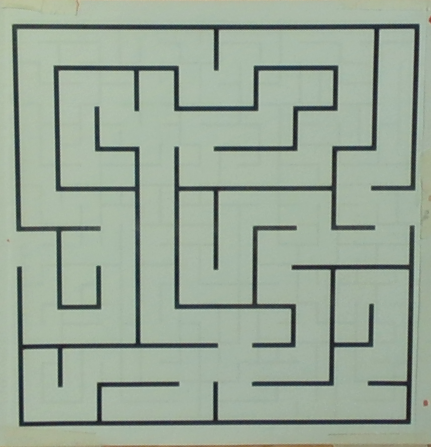
\includegraphics[width=\textwidth]{maze_rectified.png}
\caption{Rectified and cropped maze after the homography.}
\end{subfigure}
\caption{Maze localization. Left: raw capture with tag detections. Right: the flattened maze used for planning.}
\label{fig:localization}
\end{figure}

After rectification we still need a metric scale. The physical tag side length $L$ is known, 42.86,mm. We measure the average tag edge length $\bar{e}$ in rectified pixels and get the scale
\begin{equation}
s = \frac{L}{\bar{e}} \quad \left[\frac{\text{m}}{\text{px}}\right].
\end{equation}
Since the homography makes the scale uniform across the sheet, a single scalar fully determines the metric mapping. On our captures $s \approx 0.69$,mm/px, which gave a measured maze size of about $291 \times 299$,mm. The scale was repeatable to within $0.01\%$ between captures.

\subsection{Path Planning with A*}

The rectified maze image is turned into a $120 \times 120$ grid of nodes. A node is free if enough of the pixels in its cell are brighter than a threshold, corresponding to paper, and blocked otherwise, corresponding to wall. Walls are inflated by 6,px before sampling so the planned path keeps a safety margin from the walls; this matters because the pen has physical width.

The maze entrance and exit are found automatically. We scan each side of the image for places where the outer wall line dips inward, indicating a gap. Each candidate gap is then validated with a probe along the inward normal: a real opening has a free corridor leading into the maze, while artifacts from glare, shadows, or the sheet margin have wall pixels just inside them. Only validated openings are kept. A* then searches the grid from the entrance node to the exit node using an octile-distance heuristic.

\begin{figure}[H]
\centering

\includegraphics[width=0.55\textwidth]{astar_overlay.png}
\caption{A* solution overlaid on the maze. Green is the entrance, or start, and blue is the exit, or goal.}
\label{fig:astar}
\end{figure}

The raw A* path is piecewise linear and has sharp corners. We smooth it with a spline fitted through every third path node, sampled densely along its length. The spline is what the robot will actually draw.

\begin{figure}[H]
\centering

\includegraphics[width=0.55\textwidth]{astar_spline_overlay.png}
\caption{Smoothed spline, shown in magenta, through the A* path. This is the curve sent to the robot.}
\label{fig:spline}
\end{figure}

\subsection{Coordinate Frames and Transformations}

The pipeline moves every point through four frames: rectified image pixels $\rightarrow$ maze frame, metric and on the paper, $\rightarrow$ anchor tag frame $\rightarrow$ robot base frame. All rigid transforms are homogeneous matrices
\begin{equation}
T = \begin{bmatrix} R & \mathbf{p} \ \mathbf{0}^T & 1 \end{bmatrix} \in SE(3),
\qquad R \in SO(3), ; \mathbf{p} \in \mathbb{R}^3 .
\end{equation}

A spline point $(u, v)$ in rectified pixels is first scaled to metric maze coordinates using the tag-derived scale,
\begin{equation}
\mathbf{p}*{maze} = \begin{bmatrix} u,s \ v,s \ 0 \ 1 \end{bmatrix},
\end{equation}
with the maze origin at the top-left corner of the rectified crop and $z = 0$ on the paper. The point is then carried into the robot base frame through the chain
\begin{equation}
\mathbf{p}*{base} = \underbrace{T_{base \leftarrow tag}}*{\text{measured}} ;
\underbrace{T*{tag \leftarrow maze}}*{\text{measured}} ;
\mathbf{p}*{maze},
\end{equation}
where $T_{base \leftarrow tag}$ is the pose of the anchor AprilTag in the robot base frame and $T_{tag \leftarrow maze}$ is the offset from that tag to the maze origin; both were measured physically on the workcell. One axis calibration is folded into this chain: the maze image $x$ axis, columns to the right, points along negative base $x$ in our workcell layout, so the first column of $T_{base \leftarrow maze}$ is negated. The drawing height is enforced by replacing $z$ with the measured paper-plane height in the base frame, and the tool orientation is held constant, pen pointing straight down, expressed as a fixed rotation $R_{down}$.

The robot is commanded at the pen tip, not the flange. With $T_{base \leftarrow tcp}(q) = \mathrm{FK}(q)$ the forward kinematics of the arm and $T_{tcp \leftarrow pen}$ the fixed pen tool transform, the pen pose is
\begin{equation}
T_{base \leftarrow pen}(q) = \mathrm{FK}(q) ; T_{tcp \leftarrow pen}.
\end{equation}
For each Cartesian waypoint we build the desired pen pose $T^{des}*{base \leftarrow pen} = (R*{down}, \mathbf{p}*{base})$ and solve
\begin{equation}
\mathrm{FK}(q) = T^{des}*{base \leftarrow pen} ; T_{tcp \leftarrow pen}^{-1}
\end{equation}
for $q$ with the closed-form UR10e inverse kinematics. The UR10e IK has up to eight solution branches; we select a consistent elbow-up branch for every waypoint so the arm configuration never flips mid-path. The resulting joint trajectory is validated by running it back through the forward kinematics and checking that the reconstructed pen path matches the planned Cartesian path.

The IK output points are evenly spaced in pixels, but the pixel-to-joint map is nonlinear, so they are \emph{not} evenly spaced in joint space. Since the controller consumes exactly one point per control period $\Delta t$, the spacing between points sets the speed. We therefore resample the joint path to uniform joint-space arc length. With total path length $\mathcal{L} = \sum_k \lVert q_{k+1} - q_k \rVert$ and a chosen cruise speed $v_c$, the number of points is
\begin{equation}
N_{pts} = \left\lceil \frac{\mathcal{L}}{v_c , \Delta t} \right\rceil,
\end{equation}
and the trajectory is interpolated at uniform arc-length steps. After this step the commanded joint speed is constant along the whole path, which removed large reference acceleration spikes we measured before the change.

\subsection{Robot Control}

The original control plan was to track the joint-space drawing trajectory with a model predictive controller. The robot accepts joint velocity commands through \texttt{speedj}, so the planned controller modeled each joint as a single integrator,
\begin{equation}
q_{k+1} = q_k + \Delta t , u_k, \qquad q, u \in \mathbb{R}^6,
\end{equation}
with $\Delta t = 1/75$,s. At every control step the MPC was intended to solve
\begin{equation}
\begin{aligned}
  \min_{u_0, \dots, u_{N-1}} \quad
  & \sum_{t=0}^{N-1} \Big[
      (q_t - q_t^r)^T Q \,(q_t - q_t^r)
      + (u_t - u_t^r)^T R \,(u_t - u_t^r)
    \Big] \\
  & \quad + (q_N - q_N^r)^T P \,(q_N - q_N^r) \\
  \text{s.t.} \quad
  & q_{t+1} = q_t + \Delta t\,u_t, \qquad q_0 = q_{meas}, \\
  & |u_t| \le v_{max}, \qquad
    \left| \frac{u_t - u_{t-1}}{\Delta t} \right| \le a_{max}.
\end{aligned}
\end{equation}
  with horizon $N = 6$, velocity limit $v_{max} = 0.6$,rad/s, and acceleration limit $a_{max} = 1.2$,rad/s$^2$. The reference $q^r$ was the next $N{+}1$ points of the joint trajectory. The reference velocity, or feedforward term, was the discrete derivative of the reference,
  \begin{equation}
  u_t^r = \frac{\mathrm{wrap}!\left(q_{t+1}^r - q_t^r\right)}{\Delta t},
  \end{equation}
  where $\mathrm{wrap}(\cdot)$ takes the shortest angular difference so that $2\pi$ wraparounds in the IK output do not create velocity spikes. The problem was built in CasADi as a sequential quadratic program, and only the first input $u_0$ would be sent to the robot each cycle.

We also wanted to add a safety filter to the MPC using a control barrier function. The safety requirement was that the pen should never move below the drawing plane. Let
\begin{equation}
h(q) = z_{pen}(q) - z_{plane},
\end{equation}
where $z_{pen}(q)$ is the pen-tip height from forward kinematics and $z_{plane}$ is the measured drawing-plane height. The safe set is
\begin{equation}
\mathcal{C} = {q : h(q) \ge 0}.
\end{equation}
Since the commanded input is joint velocity $u = \dot q$, the derivative of the barrier is
\begin{equation}
\dot h(q,u) = \frac{\partial z_{pen}}{\partial q}(q) u
= J_z(q)u,
\end{equation}
where $J_z(q)$ is the row of the geometric Jacobian mapping joint velocities to vertical pen-tip velocity. A first-order CBF constraint would enforce
\begin{equation}
J_z(q)u \ge -\alpha h(q),
\end{equation}
with $\alpha > 0$. This constraint would allow the pen to approach the plane, but would force the vertical velocity to become nonnegative as the pen reached the boundary $h(q)=0$. In the MPC, this would appear as an additional linear inequality on the commanded velocity at each step:
\begin{equation}
J_z(q_t)u_t + \alpha \left(z_{pen}(q_t) - z_{plane}\right) \ge 0.
\end{equation}

In practice, the MPC-based implementation did not perform well on the hardware. The outputs were unexpectedly jittery, and feeding them directly into \texttt{speedj} produced motion that was not smooth enough for reliable drawing. We spent a large amount of debugging time on the MPC, the feedback stream, and the velocity command interface, but the resulting behavior remained fragile. Rather than continue tuning a controller that was not necessary for the final demonstration, we switched to a simpler and more reliable execution method.

The final robot control method directly iterates through the resampled joint-space trajectory and sends sequential \texttt{movej()} commands. For each desired waypoint $q_k^r$, the robot is commanded to move to that joint configuration before advancing to the next point:
\begin{equation}
q_k^r \longrightarrow \texttt{movej}(q_k^r).
\end{equation}
Because the path was already smoothed in Cartesian space and resampled in joint-space arc length, this simpler position-command approach was sufficient to draw the maze solution without the unstable velocity outputs we observed from the MPC. This final approach sacrificed some feedback-control elegance, but it was much more robust for the actual hardware and project timeline.

\subsection{Execution on the Robot}

A dedicated thread talks to the robot over the \texttt{urx} interface. Static point-to-point motions, including moving to the overhead camera pose, approaching the maze start, lowering the pen, and returning home, use blocking \texttt{movej} position commands. During the drawing itself, the robot iterates through the precomputed joint trajectory and sends each waypoint as a \texttt{movej()} command. This avoids relying on high-frequency velocity streaming during the final drawing run.

Two execution details were still important during development and cost most of the debugging time:

\begin{itemize}
\item \textbf{Feedback rate.} The default position read updates at only 10,Hz. When we tested the MPC at 75,Hz, the controller saw a frozen measurement for about 7 cycles in a row, built up error, and overcorrected when the measurement finally jumped. This produced a 10,Hz sawtooth in the command and visible jitter on the arm. Switching to the 125,Hz real-time stream improved the situation, but it did not fully fix the fragility of the velocity-control approach.
\item \textbf{Streaming acceleration.} Each \texttt{speedj} message interrupts the previous one, and the robot re-accelerates toward the new velocity from the deceleration caused by the interruption. With a low acceleration setting the robot only reached a fraction of the commanded speed, which shrank the drawn path. The streaming acceleration must be high enough to reach the commanded velocity within one cycle. This issue was another reason we ultimately avoided \texttt{speedj} for the final drawing behavior.
\end{itemize}

A safety layer checks each outgoing command: predicted joint positions are tested against joint limits and a link self-collision check before the command is sent.

\section{Output}

The full system was run end to end on the real robot: capture, localization, planning, and drawing. The robot draws the solution from the entrance to the exit with the pen. A video of the complete run on the real robot is available here:
\begin{center}
\url{https://drive.google.com/file/d/1m33Bf5FJT0r0q2lxJ7RcKgt9E8qJdwQp/view?usp=sharing}
\end{center}

\section{Conclusion}

The final system was able to complete the full maze-solving pipeline on real hardware. The UR10e moved to an overhead camera pose, captured the maze, localized the paper using AprilTags, rectified the image with a homography, solved the maze with A*, smoothed the path with a spline, converted the result into the robot base frame, generated a joint-space trajectory through inverse kinematics, and physically drew the solution on the page. The result was not just an isolated planning demo or a scripted robot motion: it was an end-to-end system where perception, planning, frame transformations, inverse kinematics, and hardware execution all had to work together.

At the beginning of the project, we had a more ambitious control goal. We wanted to use an MPC controller to track the joint-space trajectory while streaming velocity commands through \texttt{speedj}. We also wanted to add a CBF-based safety filter, based on material recently covered in 233, to enforce that the pen height stayed at or above the drawing plane. In principle, this would have made the controller both trajectory-tracking and safety-aware. In practice, the MPC outputs were jittery on the real robot, and the interaction between the controller, the feedback stream, and the \texttt{speedj} interface took too long to debug under the project time constraints. We therefore switched to direct joint-space execution with sequential \texttt{movej()} commands, which was less elegant from a controls perspective but substantially more reliable for the final hardware demonstration.

The main limitation of the current system is that the maze must stay in the measured workcell location. A stronger version would allow the maze to be placed anywhere on the table, then estimate the full transform chain from the camera observation of the tags to the robot base frame at runtime. That would remove the hand-measured tag-to-base dependency and make the system more flexible. Another improvement would be faster and smoother drawing. This could come from a more robust version of the velocity-control pipeline, better trajectory timing, or a properly debugged MPC implementation with the CBF safety constraint included. Those changes would make the system less like a careful waypoint follower and more like a genuinely controlled drawing robot.

\end{document}
